\begin{frame}
  \frametitle{Datos de Contacto}
  \begin{columns}[T,onlytextwidth]
    \begin{column}{0.48\textwidth}
      \begin{block}{Oliver Pardo}
        \textit{Profesor de la clase magistral}\\[0.15cm]
        PhD en Econom\'ia, LSE\\
        Profesor Asociado, FCEA--PUJ\\[0.2cm]
        pardoo@javeriana.edu.co
      \end{block}
    \end{column}
    \begin{column}{0.48\textwidth}
      \begin{block}{Andr\'es Garz\'on}
        \textit{Profesor del taller aplicado}\\[0.15cm]
        An\'alisis de informaci\'on y datos de finanzas p\'ublicas\\[0.2cm]
        garzonandresf@javeriana.edu.co
      \end{block}
    \end{column}
  \end{columns}
  \note{[Sources] ProgramaFPC, Google Doc suministrado por el usuario, consultado el 29 de julio de 2026.}
\end{frame}


\begin{frame}
  \frametitle{Introducci\'on}
  El curso estudia c\'omo funciona y se financia el sector p\'ublico colombiano, c\'omo se asignan y ejecutan los recursos y qu\'e implicaciones tienen estas decisiones sobre:
  \begin{itemize}
    \item el desempe\~no econ\'omico y la estabilidad macroecon\'omica;
    \item la equidad y el desarrollo social;
    \item la sostenibilidad fiscal y la coordinaci\'on intergubernamental.
  \end{itemize}
  Combina teor\'ia econ\'omica, an\'alisis institucional, datos y discusi\'on de pol\'iticas p\'ublicas.
  \note{[Sources] ProgramaFPC, Google Doc suministrado por el usuario, consultado el 29 de julio de 2026.}
\end{frame}

\begin{frame}
  \frametitle{Objetivos del Curso}
  \begin{itemize}
    \item Comprender la estructura institucional y fiscal del sector p\'ublico.
    \item Analizar ingresos y gastos nacionales y territoriales.
    \item Evaluar la sostenibilidad fiscal y sus efectos macroecon\'omicos y sociales.
    \item Interpretar el MFMP, el PGN y los informes del FMI.
    \item Formular argumentos y propuestas de pol\'itica sustentados en evidencia.
    \item Manejar y visualizar datos fiscales con herramientas digitales.
  \end{itemize}
  \note{[Sources] ProgramaFPC, Google Doc suministrado por el usuario, consultado el 29 de julio de 2026.}
\end{frame}

\begin{frame}
  \frametitle{Metodolog\'ia y Evaluaci\'on}
  \begin{block}{Sesi\'on semanal: 4 horas}
    \textbf{3 horas:} clase magistral, quizzes y presentaciones, a cargo de Oliver Pardo.\\
    \textbf{1 hora:} taller de an\'alisis de informaci\'on fiscal, a cargo de Andr\'es Garz\'on.
  \end{block}
  \begin{alertblock}{Evaluaci\'on}
    \begin{itemize}
      \item \textbf{Quizzes: 33,33\%.} Lecturas, clase magistral y presentaciones.
      \item \textbf{Presentaci\'on en grupo: 33,33\%.} Equipos de 2--3 estudiantes; hasta dos horas, incluida la discusi\'on.
      \item \textbf{Taller aplicado: 33,33\%.}
    \end{itemize}
  \end{alertblock}
  \note{[Sources] ProgramaFPC, Google Doc suministrado por el usuario, consultado el 29 de julio de 2026.}
\end{frame}


\begin{frame}
  \frametitle{El curso avanza de la arquitectura fiscal a su aplicaci\'on}
  \small
  \begin{itemize}
    \item \textbf{M0:} Presentaci\'on del curso --- 1 sesi\'on
    \item \textbf{M1:} Conceptualizaci\'on del sector p\'ublico --- 1 sesi\'on
    \item \textbf{M2:} Gobierno Nacional Central --- 4 sesiones
    \item \textbf{M3:} Regla fiscal y ciclo presupuestal --- 1 sesi\'on
    \item \textbf{M4:} Seguridad social en pensiones --- 2 sesiones
    \item \textbf{M5:} Seguridad social en salud --- 1 sesi\'on
    \item \textbf{M6:} Finanzas p\'ublicas territoriales --- 1 sesi\'on
    \item \textbf{M7:} Colombia en el contexto internacional --- 1 sesi\'on
    \item \textbf{M8:} Presentaciones en grupo --- 6 sesiones
  \end{itemize}
  \note{[Sources] ProgramaFPC, Google Doc suministrado por el usuario, consultado el 29 de julio de 2026.}
\end{frame}

\begin{frame}
  \frametitle{Componente Aplicado: Manejo de Datos}
  \begin{itemize}
    \item Base de datos del Gobierno Nacional Central.
    \item PEPE: Presupuesto en Perspectiva Econ\'omica.
    \item GEIH para el an\'alisis de pensiones y protecci\'on social.
    \item SICODIS para distribuciones de recursos territoriales.
    \item Terridata y FUT para finanzas departamentales y municipales.
    \item Visualizaci\'on e interpretaci\'on de indicadores fiscales.
  \end{itemize}
  \note{[Sources] ProgramaFPC, Google Doc suministrado por el usuario, consultado el 29 de julio de 2026.}
\end{frame}

\begin{frame}{M1--M2: del mapa institucional a las cuentas del GNC}
\scriptsize
\begin{columns}[T,onlytextwidth]
  \begin{column}{0.38\textwidth}
    \begin{block}{M1. Sector p\'ublico colombiano}
      \textbf{Obligatorias}
      \begin{itemize}
        \item C\'ardenas (2020), \textit{Introducci\'on a la Econom\'ia Colombiana}, cap. 6.
        \item Lora y Prada (2023), \textit{T\'ecnicas de medici\'on econ\'omica}, cap. 17.
      \end{itemize}
      \textbf{Sugerida:} FMI (2014), \textit{Manual de Estad\'isticas de Finanzas P\'ublicas}.
    \end{block}
  \end{column}
  \begin{column}{0.35\textwidth}
    \begin{block}{M2. Gobierno Nacional Central}
      \textbf{Obligatoria}
      \begin{itemize}
        \item Pardo (2025), \textit{El Laberinto Fiscal de Colombia}, caps. 1, 2, 4, 5 y 6.
      \end{itemize}
      \textbf{Sugeridas}
      \begin{itemize}
        \item Rinc\'on-Castro y Zapata-\'Alvarez (2025).
        \item CARF (abril de 2026), \textit{Informe al Congreso}.
      \end{itemize}
      \textbf{Datos:} archivo del GNC.
    \end{block}
  \end{column}
  \begin{column}{0.20\textwidth}
    \centering
    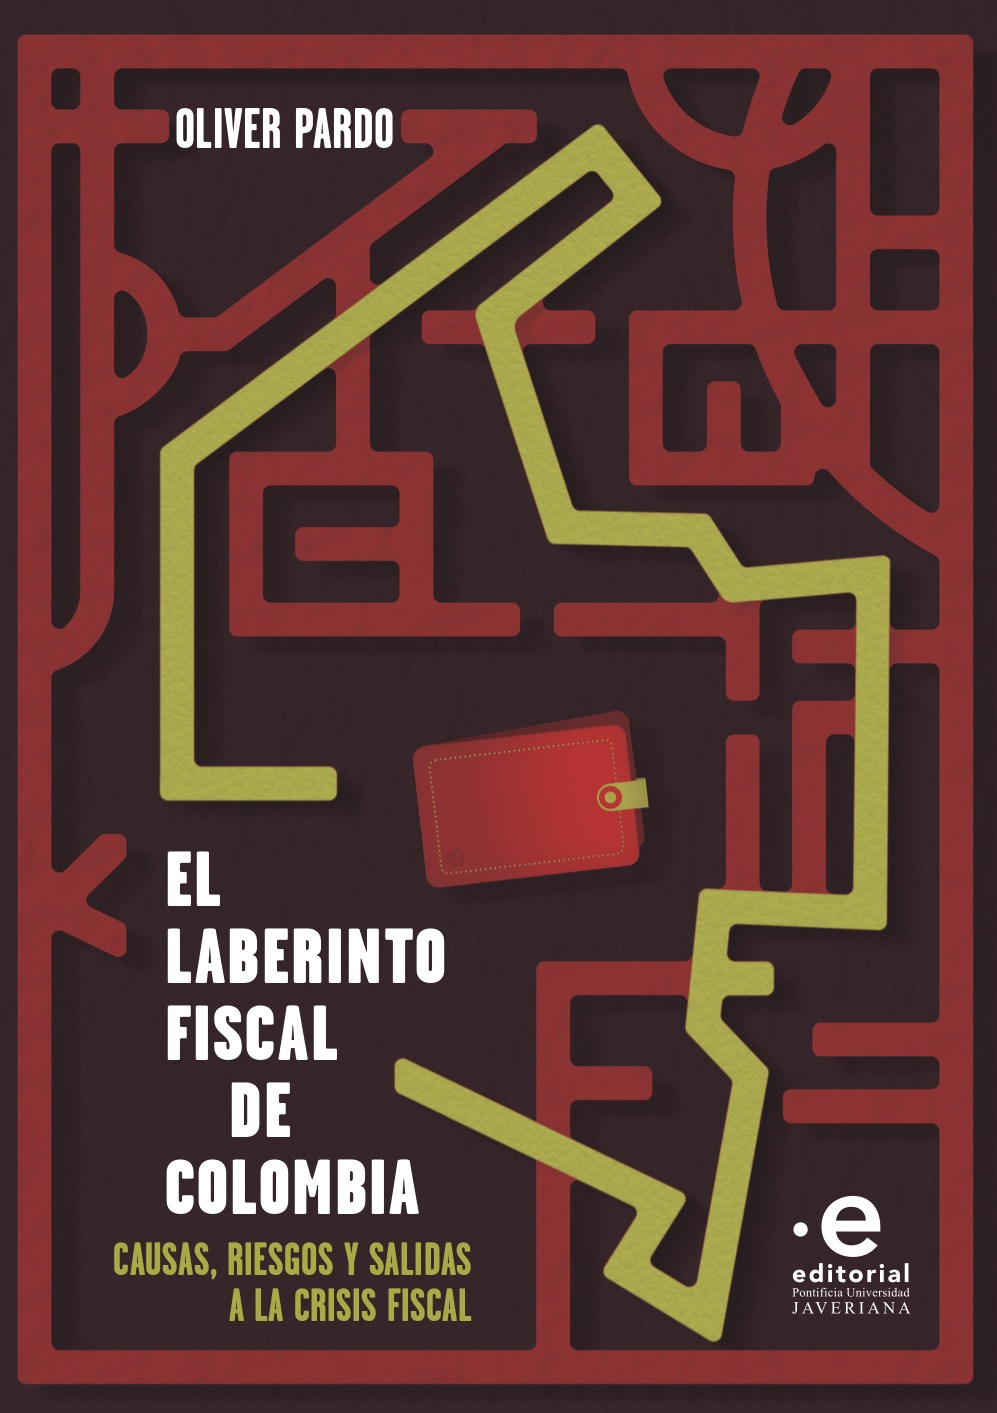
\includegraphics[width=\linewidth]{assets/laberinto_fiscal_portada.jpg}\\[-0.05cm]
    \tiny Editorial Javeriana, 2025
  \end{column}
\end{columns}
\note{[Sources] ProgramaFPC, Google Doc suministrado por el usuario, consultado el 29 de julio de 2026. Portada: Editorial Pontificia Universidad Javeriana, \href{https://www.javeriana.edu.co/web/editorial/w/laberinto-fiscal-colombia}{El laberinto fiscal de Colombia}.}
\end{frame}

\begin{frame}{M3: las reglas conectan el presupuesto con la sostenibilidad}
\footnotesize
\begin{block}{Lecturas obligatorias}
  \begin{itemize}
    \item L\'opez Velandia y L\'opez Ghio (2019), \textit{Regla fiscal para el gobierno central en Colombia}.
    \item FMI (2022), \textit{Fiscal Rules and Fiscal Councils: Recent Trends and Performance during the COVID-19 Pandemic}.
  \end{itemize}
\end{block}
\begin{block}{Lecturas sugeridas}
  \begin{itemize}
    \item Ministerio de Hacienda: MFMP 2026 e informe de cumplimiento de la regla fiscal 2025.
    \item Observatorio Fiscal PUJ: \textit{As\'i funciona el Presupuesto General de la Naci\'on}.
    \item Pardo (2025), \textit{El Laberinto Fiscal de Colombia}, cap. 3.
  \end{itemize}
\end{block}
\begin{alertblock}{Aplicaci\'on}
Herramienta PEPE: Presupuesto en Perspectiva Econ\'omica, Observatorio Fiscal PUJ.
\end{alertblock}
\note{[Sources] ProgramaFPC, Google Doc suministrado por el usuario, consultado el 29 de julio de 2026.}
\end{frame}

\begin{frame}{M4--M5: la seguridad social tambi\'en es pol\'itica fiscal}
\scriptsize
\begin{columns}[T,onlytextwidth]
  \begin{column}{0.49\textwidth}
    \begin{block}{M4. Pensiones}
      \textbf{Lecturas obligatorias}
      \begin{itemize}
        \item Observatorio Fiscal PUJ, \textit{Gu\'ia Ciudadana al Sistema de Pensiones y la Protecci\'on de la Vejez}.
        \item Observatorio Fiscal PUJ, \textit{Primer an\'alisis del Proyecto de Reforma Pensional}.
        \item Hartmann y Pardo, \textit{C\'omo financiar el Pilar Solidario sin reventar el Presupuesto}.
      \end{itemize}
      \textbf{Datos:} introducci\'on y uso de la GEIH.
    \end{block}
  \end{column}
  \begin{column}{0.49\textwidth}
    \begin{block}{M5. Salud}
      \textbf{Lecturas obligatorias}
      \begin{itemize}
        \item Observatorio Fiscal PUJ, \textit{Gu\'ia Ciudadana al Sistema de Salud}.
        \item ACEMI (2026), propuestas para la estabilizaci\'on y fortalecimiento del sistema de salud 2026--2030.
      \end{itemize}
      \textbf{Datos:} introducci\'on y uso de SICODIS.
    \end{block}
  \end{column}
\end{columns}
\note{[Sources] ProgramaFPC, Google Doc suministrado por el usuario, consultado el 29 de julio de 2026.}
\end{frame}

\begin{frame}{M6 y M7: territorio y comparaci\'on internacional}
\scriptsize
\begin{columns}[T,onlytextwidth]
  \begin{column}{0.57\textwidth}
    \begin{block}{M6. Finanzas p\'ublicas territoriales}
      \textbf{Obligatorias}
      \begin{itemize}
        \item Observatorio Fiscal PUJ, \textit{¿De d\'onde vienen y hacia d\'onde van los recursos de mi municipio?}
        \item Comisi\'on de Estudio del Sistema Tributario Territorial (2020), \textit{Informe Final}.
      \end{itemize}
      \textbf{Sugeridas}
      \begin{itemize}
        \item Carreri y Martinez (2023), reglas fiscales y rendici\'on de cuentas.
        \item \textit{A subnational resource curse?}
      \end{itemize}
      \textbf{Datos:} Terridata y FUT.
    \end{block}
  \end{column}
  \begin{column}{0.40\textwidth}
    \begin{block}{M7. Contexto internacional}
      \textbf{Lectura obligatoria}\\[0.15cm]
      FMI, \textit{Colombia: 2024 Article IV Consultation---Staff Report}.
    \end{block}
    \begin{alertblock}{Pregunta transversal}
      ¿En qu\'e se parece y en qu\'e se diferencia Colombia de otras econom\'ias comparables?
    \end{alertblock}
  \end{column}
\end{columns}
\note{[Sources] ProgramaFPC, Google Doc suministrado por el usuario, consultado el 29 de julio de 2026.}
\end{frame}

\begin{frame}{M8: la presentaci\'on debe conducir a una discusi\'on}
\small
\begin{block}{Formato}
  Grupos de 2--3 estudiantes. La sesi\'on puede durar hasta dos horas y debe reservar al menos una hora para discusi\'on.
\end{block}
\begin{columns}[T,onlytextwidth]
  \begin{column}{0.48\textwidth}
    \begin{itemize}
      \item Crisis fiscal
      \item Crisis del sistema de salud
      \item Reforma pensional
      \item Cajas de compensaci\'on
      \item Ecopetrol
    \end{itemize}
  \end{column}
  \begin{column}{0.48\textwidth}
    \begin{itemize}
      \item Pol\'itica monetaria y dominancia fiscal
      \item Finanzas de una entidad territorial
      \item Renta de personas jur\'idicas
      \item Renta de personas naturales
      \item Reforma al IVA
    \end{itemize}
  \end{column}
\end{columns}
\note{[Sources] ProgramaFPC, Google Doc suministrado por el usuario, consultado el 29 de julio de 2026.}
\end{frame}

\begin{frame}{M8: coyuntura, presupuesto y territorio}
\small
\begin{columns}[T,onlytextwidth]
  \begin{column}{0.48\textwidth}
    \begin{itemize}
      \item Ejecuci\'on del PGN 2025
      \item PGN 2026
      \item PGN 2027
      \item MFMP 2026
      \item Ejecuci\'on del presupuesto de regal\'ias 2023--2024
    \end{itemize}
  \end{column}
  \begin{column}{0.48\textwidth}
    \begin{itemize}
      \item Formulaci\'on del presupuesto de regal\'ias 2025--2026
      \item Art\'iculo IV del FMI
      \item Catastro multiprop\'osito
      \item Activaci\'on de la cl\'ausula de escape
      \item Otro tema fiscal acordado con el profesor
    \end{itemize}
  \end{column}
\end{columns}
\begin{alertblock}{Criterio}
El listado no es exhaustivo: un grupo puede proponer otro tema y solicitar referencias al profesor.
\end{alertblock}
\note{[Sources] ProgramaFPC, Google Doc suministrado por el usuario, consultado el 29 de julio de 2026.}
\end{frame}

\begin{frame}
  \frametitle{Funciones del Estado y su Base Constitucional}
  \begin{itemize}
    \item \textbf{Legislativa:} Crear leyes (Art. 1, 3)
    \item \textbf{Ejecutiva:} Administrar y ejecutar leyes (Art. 113, 209)
    \item \textbf{Judicial:} Aplicar justicia (Art. 229, 228)
    \item \textbf{Defensa y seguridad:} Proteger soberan\'ia y orden (Art. 2)
    \item \textbf{Econ\'omica:} Dirigir la econom\'ia y corregir desigualdades (Art. 1, 334)
    \item \textbf{Social:} Garantizar derechos b\'asicos (Art. 1, 2, 366)
    \item \textbf{Fiscal:} Recaudar y asignar recursos (Art. 338, 95)
    \item \textbf{Reguladora:} Supervisar mercados y servicios (Art. 333, 365)
  \end{itemize}
\end{frame}

\begin{frame}
  \frametitle{Art\'iculo 1 - CP de 1991}
  Colombia es un Estado social de derecho, organizado en forma de Rep\'ublica unitaria, descentralizada, con autonom\'ia de sus entidades territoriales, democr\'atica, participativa y pluralista, fundada en el respeto de la dignidad humana, en el trabajo y la solidaridad de las personas que la integran y en la prevalencia del inter\'es general.
\end{frame}

\begin{frame}
  \frametitle{Art\'iculo 2 - CP de 1991}
  Son fines esenciales del Estado: servir a la comunidad, promover la prosperidad general y garantizar la efectividad de los principios, derechos y deberes consagrados en la Constituci\'on; facilitar la participaci\'on de todos en las decisiones que los afectan y en la vida econ\'omica, pol\'itica, administrativa y cultural de la Naci\'on; defender la independencia nacional, mantener la integridad territorial y asegurar la convivencia pac\'ifica y la vigencia de un orden justo.
\end{frame}

\begin{frame}
  \frametitle{Art\'iculo 3 - CP de 1991}
  La soberan\'ia reside exclusivamente en el pueblo, del cual emana el poder p\'ublico. El pueblo la ejerce en forma directa o por medio de sus representantes, en los t\'erminos que la Constituci\'on establece.
\end{frame}

\begin{frame}
  \frametitle{Art\'iculo 95 - CP de 1991}
  La constituci\'on establece como deber de la persona y del ciudadano contribuir al financiamiento de los gastos e inversiones del Estado dentro de conceptos de justicia y equidad.
\end{frame}

\begin{frame}
  \frametitle{Art\'iculo 113 - CP de 1991}
  Son ramas del poder p\'ublico la legislativa, la ejecutiva y la judicial. Adem\'as de los \'organos que las integran, existen otros, aut\'onomos e independientes, para el cumplimiento de las funciones del Estado. Los diferentes \'organos del Estado tienen funciones separadas pero colaboran arm\'onicamente para la realizaci\'on de sus fines.
\end{frame}

\begin{frame}{El Estado es m\'as amplio que las tres ramas}
\scriptsize
\begin{columns}[T,onlytextwidth]
  \begin{column}{0.32\textwidth}
    \begin{block}{Rama legislativa}
      \textbf{Congreso de la Rep\'ublica}
      \begin{itemize}
        \item Senado
        \item C\'amara de Representantes
      \end{itemize}
      Hace las leyes, reforma la Constituci\'on y ejerce control pol\'itico.
    \end{block}
  \end{column}
  \begin{column}{0.32\textwidth}
    \begin{block}{Rama ejecutiva}
      \textbf{Orden nacional}
      \begin{itemize}
        \item Presidencia
        \item Sectores (Hacienda, Defensa, Salud, etc)
      \end{itemize}
      \textbf{Orden territorial:} Gobernaciones y Alcald\'ias.
    \end{block}
  \end{column}
  \begin{column}{0.32\textwidth}
    \begin{block}{Rama judicial}
      \begin{itemize}
        \item Corte Constitucional
        \item Corte Suprema 
        %\item Consejo de Estado
        \item Fiscal\'ia General
        \item Tribunales y juzgados
        %\item Gobierno y disciplina judicial
      \end{itemize}
    \end{block}
  \end{column}
\end{columns}
\vspace{0.15cm}
\begin{alertblock}{Organismos autónomos}
 Contralor\'ia y Procuraduría.
\quad  CNE y Registradur\'ia.
\quad Banco de la Rep\'ublica.
\end{alertblock}
\note{[Sources] Constituci\'on Pol\'itica de Colombia, arts. 113--120, 249, 265--266, 267, 275, 371 y 130. Texto oficial: Secretar\'ia del Senado.}
\end{frame}

\begin{frame}{La separaci\'on es funcional, no aislamiento}
\small
\begin{tabular}{p{0.19\textwidth}p{0.36\textwidth}p{0.36\textwidth}}
\textbf{Rama} & \textbf{Funci\'on principal} & \textbf{Ejemplo fiscal} \\ \hline
\textbf{Legislativa} &
Expide leyes, reforma la Constituci\'on y controla pol\'iticamente al Gobierno. &
Aprueba tributos, presupuesto y endeudamiento dentro de sus competencias. \\[0.18cm]
\textbf{Ejecutiva} &
Formula pol\'iticas, administra y reglamenta las leyes sin sustituir al legislador. &
Presenta el presupuesto, recauda, ejecuta el gasto y expide decretos reglamentarios. \\[0.18cm]
\textbf{Judicial} &
Resuelve controversias y controla la constitucionalidad o legalidad seg\'un la jurisdicci\'on. &
Puede retirar o suspender normas fiscales incompatibles con normas superiores. \\
\end{tabular}
\vspace{0.25cm}
\begin{block}{Regla de lectura}
Las funciones est\'an separadas, pero los \'organos colaboran arm\'onicamente y se controlan entre s\'i. La competencia concreta siempre depende de la Constituci\'on y la ley. En la práctica, habrán controversias.
\end{block}
\note{[Sources] Constituci\'on Pol\'itica, arts. 113--116, 150, 189, 241 y 237.}
\end{frame}

\begin{frame}{Jerarqu\'ia normativa: qui\'en expide y qui\'en modifica}
\scriptsize
\begin{tabular}{p{0.22\textwidth}p{0.31\textwidth}p{0.38\textwidth}}
\textbf{Nivel} & \textbf{Qui\'en la expide} & \textbf{C\'omo se modifica o controla} \\ \hline
\textbf{Constituci\'on} &
Pueblo constituyente; Congreso mediante acto legislativo. &
Acto legislativo, referendo o asamblea constituyente. La Corte controla los procedimientos de reforma. \\[0.16cm]
\textbf{Leyes} &
Congreso; el Presidente sanciona y promulga. &
Otra ley del tipo y tr\'amite exigidos. La Corte Constitucional puede declarar su inexequibilidad. \\[0.16cm]
\textbf{Decretos con fuerza de ley} &
Gobierno por habilitaci\'on constitucional: facultades extraordinarias o estados de excepci\'on. &
El Congreso puede modificarlos por ley dentro de sus competencias; la Corte controla sus l\'imites de materia, tiempo y procedimiento. \\[0.16cm]
\textbf{Decretos reglamentarios} &
Presidente y Gobierno para ejecutar la ley. &
No pueden crear ni modificar la ley. El Gobierno puede derogarlos y la jurisdicci\'on contenciosa controla su legalidad. \\[0.16cm]
\textbf{Actos administrativos} &
Ministros y otras autoridades: resoluciones, circulares y \'ordenes, seg\'un competencia. &
Deben respetar Constituci\'on, ley y reglamentos superiores; pueden ser revocados o anulados conforme al ordenamiento. \\
\end{tabular}
\vspace{0.12cm}
%\textit{Precisi\'on:} no existe una pir\'amide exhaustiva y lineal para todas las normas. Importan tambi\'en la materia, la competencia y los procedimientos especiales.
\note{[Sources] Constituci\'on Pol\'itica, arts. 4, 150, 189.10--11, 212--215, 241 y 374--379; Corte Constitucional, sentencias C-037 de 2000 y C-536 de 2005.}
\end{frame}

%\begin{frame}{Los contrapesos operan antes y despu\'es de decidir}
%\small
%\begin{tikzpicture}[
%  node distance=1.3cm and 1.5cm,
%  organ/.style={rectangle, rounded corners, draw=blue!70, fill=blue!8,
%    text width=3.0cm, minimum height=1.05cm, align=center},
%  control/.style={-{Stealth[length=2mm]}, thick, draw=black!65}
%]
%  \node[organ] (congreso) {\textbf{Congreso}\\leyes, presupuesto\\y control pol\'itico};
%  \node[organ, right=of congreso] (gobierno) {\textbf{Gobierno}\\sanci\'on u objeci\'on\\y ejecuci\'on};
%  \node[organ, below=of congreso] (corte) {\textbf{Corte Constitucional}\\control de la ley y de\\decretos con fuerza de ley};
%  \node[organ, right=of corte] (consejo) {\textbf{Consejo de Estado}\\control de actos\\administrativos};

%  \draw[control, bend left=12] (congreso) to node[above, sloped, font=\tiny]{autoriza y controla} (gobierno);
%  \draw[control, bend left=12] (gobierno) to node[below, sloped, font=\tiny]{sanciona u objeta} (congreso);
%  \draw[control] (corte) -- node[left, font=\tiny]{constitucionalidad} (congreso);
%  \draw[control] (corte) -- node[below, sloped, font=\tiny]{l\'imites constitucionales} (gobierno);
%  \draw[control] (consejo) -- node[right, font=\tiny]{legalidad} (gobierno);
%\end{tikzpicture}
%\vspace{0.15cm}
%\begin{alertblock}{Controles transversales}
%Contralor\'ia: control fiscal. %Procuraduría: vigilancia disciplinaria y protecci\'on de derechos; 
%Ciudadan\'ia: voto, tutela y derechos de petición.
%\end{alertblock}
%\note{[Sources] Constituci\'on Pol\'itica, arts. 113, 135, 150, 167, 189, 237, 241, 267 y 275--282.}
%\end{frame}

\begin{frame}
  \frametitle{Art\'iculo 209 - CP de 1991}
  La funci\'on administrativa est\'a al servicio de los intereses generales y se desarrolla con fundamento en los principios de igualdad, moralidad, eficacia, econom\'ia, celeridad, imparcialidad y publicidad, mediante la descentralizaci\'on, la delegaci\'on y la desconcentraci\'on de funciones.
\end{frame}

\begin{frame}
  \frametitle{Art\'iculo 228 - CP de 1991}
  La administraci\'on de justicia es funci\'on p\'ublica. Sus decisiones son independientes. Las actuaciones ser\'an p\'ublicas y permanentes, con las excepciones que establezca la ley, y los t\'erminos procesales se observar\'an con diligencia. Su funcionamiento ser\'a desconcentrado y aut\'onomo.
\end{frame}

\begin{frame}
  \frametitle{Art\'iculo 229 - CP de 1991}
  Se garantiza el derecho de toda persona para acceder a la administraci\'on de justicia. La ley indicar\'a en qu\'e casos puede hacerlo sin la representaci\'on de abogado.
\end{frame}

\begin{frame}
  \frametitle{Art\'iculo 333 - CP de 1991}
  La actividad econ\'omica y la iniciativa privada son libres, dentro de los l\'imites del bien com\'un. La empresa, como base del desarrollo, tiene una funci\'on social que implica obligaciones. El Estado, por mandato de la ley, intervendr\'a por razones de utilidad p\'ublica o de inter\'es social.
\end{frame}

\begin{frame}
  \frametitle{Art\'iculo 334 - CP de 1991}
  El Estado intervendr\'a por mandato de la ley en la explotaci\'on de los recursos naturales, en el uso del suelo, en la producci\'on, distribuci\'on, utilizaci\'on y consumo de los bienes, y en los servicios p\'ublicos y privados, para racionalizar la econom\'ia con el fin de conseguir el mejoramiento de la calidad de vida.
\end{frame}

\begin{frame}
  \frametitle{Art\'iculo 338 - CP de 1991}
  En tiempo de paz, solamente el Congreso, las asambleas departamentales y los concejos distritales y municipales podr\'an imponer contribuciones fiscales o parafiscales. La ley, las ordenanzas y los acuerdos deben fijar directamente los sujetos activos y pasivos, los hechos y las bases gravables, y las tarifas de los impuestos.
\end{frame}

\begin{frame}
  \frametitle{Art\'iculo 365 - CP de 1991}
  Los servicios p\'ublicos son inherentes a la finalidad social del Estado. Es deber del Estado asegurar su prestaci\'on eficiente a todos los habitantes del territorio nacional. Podr\'an ser prestados por el Estado, directa o indirectamente, por comunidades organizadas, o por particulares.
\end{frame}

\begin{frame}
  \frametitle{Art\'iculo 366 - CP de 1991}
  El bienestar general y el mejoramiento de la calidad de vida de la poblaci\'on son finalidades sociales del Estado. Ser\'a objetivo fundamental de su actividad la soluci\'on de las necesidades insatisfechas de salud, de educaci\'on, de saneamiento ambiental y de agua potable.
\end{frame}


\begin{frame}
  \frametitle{Funciones del Estado y su Base Constitucional}
  \begin{itemize}
    \item \textbf{Legislativa:} Crear leyes (Art. 1, 3)
    \item \textbf{Ejecutiva:} Administrar y ejecutar leyes (Art. 113, 209)
    \item \textbf{Judicial:} Aplicar justicia (Art. 229, 228)
    \item \textbf{Defensa y seguridad:} Proteger soberan\'ia y orden (Art. 2)
    \item \textbf{Econ\'omica:} Dirigir la econom\'ia y corregir desigualdades (Art. 1, 334)
    \item \textbf{Social:} Garantizar derechos b\'asicos (Art. 1, 2, 366)
    \item \textbf{Fiscal:} Recaudar y asignar recursos (Art. 338, 95)
    \item \textbf{Reguladora:} Supervisar mercados y servicios (Art. 333, 365)
  \end{itemize}
\end{frame}

\begin{frame}{Desagregaci\'on del Sector P\'ublico Consolidado}
\centering
\begin{tikzpicture}[node distance=0.5cm and 0.5cm, every node/.style={align=center},
  box/.style={rectangle, draw, rounded corners, text width=3cm, minimum height=0.7cm},
  level/.style={rectangle, draw, text width=3cm, minimum height=0.7cm}]

\node[box, fill=blue!10] (spc) {\tiny{Sector P\'ublico Consolidado}};

\node[level, below left=of spc] (spf) {\tiny{Sector Público Financiero}};
\node[level, fill=green!10, below =of spc] (spnf) {\tiny{Sector Público No Financiero}};


\node[level, fill=green!10, below=of spnf] (gg) {\tiny{Gobierno General}};
\node[level, below left =of spnf] (eepp) {\tiny{Empresas Públicas}};


\node[level, fill=red!10, below left=of gg] (gnc) {\tiny{Gobierno Nacional Central}};
\node[level, fill=red!10, below =of gg] (et) {\tiny{Entidades Territoriales}};
\node[level, fill=red!10, below right =of gg] (ss) {\tiny{Seguridad Social}};

%\node[level, below left=of ss] (salud) {\tiny{Salud}};
%\node[level, below right =of ss] (pensiones) {\tiny{Pensiones}};

\node[box, fill=blue!10] (spc) {Sector P\'ublico Consolidado};

% Conexiones directas desde SPC
\draw[->] (spc) -- (spf);
\draw[->] (spc) -- (spnf);

\draw[->] (spnf) -- (gg);
\draw[->] (spnf) -- (eepp);

\draw[->] (gg) -- (gnc);
\draw[->] (gg) -- (et);
\draw[->] (gg) -- (ss);
\end{tikzpicture}
\end{frame}


